
%% bare_jrnl.tex
%% V1.4b
%% 2015/08/26
%% by Michael Shell
%% see http://www.michaelshell.org/
%% for current contact information.
%%
%% This is a skeleton file demonstrating the use of IEEEtran.cls
%% (requires IEEEtran.cls version 1.8b or later) with an IEEE
%% journal paper.
%%
%% Support sites:
%% http://www.michaelshell.org/tex/ieeetran/
%% http://www.ctan.org/pkg/ieeetran
%% and
%% http://www.ieee.org/

%%*************************************************************************
%% Legal Notice:
%% This code is offered as-is without any warranty either expressed or
%% implied; without even the implied warranty of MERCHANTABILITY or
%% FITNESS FOR A PARTICULAR PURPOSE! 
%% User assumes all risk.
%% In no event shall the IEEE or any contributor to this code be liable for
%% any damages or losses, including, but not limited to, incidental,
%% consequential, or any other damages, resulting from the use or misuse
%% of any information contained here.
%%
%% All comments are the opinions of their respective authors and are not
%% necessarily endorsed by the IEEE.
%%
%% This work is distributed under the LaTeX Project Public License (LPPL)
%% ( http://www.latex-project.org/ ) version 1.3, and may be freely used,
%% distributed and modified. A copy of the LPPL, version 1.3, is included
%% in the base LaTeX documentation of all distributions of LaTeX released
%% 2003/12/01 or later.
%% Retain all contribution notices and credits.
%% ** Modified files should be clearly indicated as such, including  **
%% ** renaming them and changing author support contact information. **
%%*************************************************************************


% *** Authors should verify (and, if needed, correct) their LaTeX system  ***
% *** with the testflow diagnostic prior to trusting their LaTeX platform ***
% *** with production work. The IEEE's font choices and paper sizes can   ***
% *** trigger bugs that do not appear when using other class files.       ***                          ***
% The testflow support page is at:
% http://www.michaelshell.org/tex/testflow/



\documentclass[12pt, conference]{IEEEtran}
%
% If IEEEtran.cls has not been installed into the LaTeX system files,
% manually specify the path to it like:
% \documentclass[journal]{../sty/IEEEtran}

\usepackage{hyperref}
\usepackage{filecontents}

\begin{filecontents*}{references.bib}
@article{reiss2019deep,
  title={Deep ppg: Large-scale heart rate estimation with convolutional neural networks},
  author={Reiss, Attila and Indlekofer, Ina and Schmidt, Philip and Van Laerhoven, Kristof},
  journal={Sensors},
  volume={19},
  number={14},
  pages={3079},
  year={2019},
  publisher={Multidisciplinary Digital Publishing Institute}
}

@article{salehizadeh2016novel,
  title={A novel time-varying spectral filtering algorithm for reconstruction of motion artifact corrupted heart rate signals during intense physical activities using a wearable photoplethysmogram sensor},
  author={Salehizadeh, Seyed and Dao, Duy and Bolkhovsky, Jeffrey and Cho, Chae and Mendelson, Yitzhak and Chon, Ki H},
  journal={Sensors},
  volume={16},
  number={1},
  pages={10},
  year={2016},
  publisher={Multidisciplinary Digital Publishing Institute}
}

@article{brophy2020optimised,
  title={Optimised convolutional neural networks for heart rate estimation and human activity recognition in wrist worn sensing applications},
  author={Brophy, Eoin and Muehlhausen, Willie and Smeaton, Alan F and Ward, Tomas E},
  journal={arXiv preprint arXiv:2004.00505},
  year={2020}
}

@article{biswas2019cornet,
  title={CorNET: Deep learning framework for PPG-based heart rate estimation and biometric identification in ambulant environment},
  author={Biswas, Dwaipayan and Everson, Luke and Liu, Muqing and Panwar, Madhuri and Verhoef, Bram-Ernst and Patki, Shrishail and Kim, Chris H and Acharyya, Amit and Van Hoof, Chris and Konijnenburg, Mario and others},
  journal={IEEE transactions on biomedical circuits and systems},
  volume={13},
  number={2},
  pages={282--291},
  year={2019},
  publisher={IEEE}
}

@article{panwar2020pp,
  title={PP-Net: A Deep Learning Framework for PPG-Based Blood Pressure and Heart Rate Estimation},
  author={Panwar, Madhuri and Gautam, Arvind and Biswas, Dwaipayan and Acharyya, Amit},
  journal={IEEE Sensors Journal},
  volume={20},
  number={17},
  pages={10000--10011},
  year={2020},
  publisher={IEEE}
}

@article{chang2021deepheart,
  title={DeepHeart: A Deep Learning Approach for Accurate Heart Rate Estimation from PPG Signals},
  author={Chang, Xiangmao and Li, Gangkai and Xing, Guoliang and Zhu, Kun and Tu, Linlin},
  journal={ACM Transactions on Sensor Networks (TOSN)},
  volume={17},
  number={2},
  pages={1--18},
  year={2021},
  publisher={ACM New York, NY, USA}
}

@article{biswas2019heart,
  title={Heart rate estimation from wrist-worn photoplethysmography: A review},
  author={Biswas, Dwaipayan and Sim{\~o}es-Capela, Neide and Van Hoof, Chris and Van Helleputte, Nick},
  journal={IEEE Sensors Journal},
  volume={19},
  number={16},
  pages={6560--6570},
  year={2019},
  publisher={IEEE}
}

@article{kingma2014adam,
  title={Adam: A method for stochastic optimization},
  author={Kingma, Diederik P and Ba, Jimmy},
  journal={arXiv preprint arXiv:1412.6980},
  year={2014}
}

@article{lundberg2017unified,
  title={A unified approach to interpreting model predictions},
  author={Lundberg, Scott and Lee, Su-In},
  journal={arXiv preprint arXiv:1705.07874},
  year={2017}
}


\end{filecontents*}


% Some very useful LaTeX packages include:
% (uncomment the ones you want to load)


% *** MISC UTILITY PACKAGES ***
%
%\usepackage{ifpdf}
% Heiko Oberdiek's ifpdf.sty is very useful if you need conditional
% compilation based on whether the output is pdf or dvi.
% usage:
% \ifpdf
%   % pdf code
% \else
%   % dvi code
% \fi
% The latest version of ifpdf.sty can be obtained from:
% http://www.ctan.org/pkg/ifpdf
% Also, note that IEEEtran.cls V1.7 and later provides a builtin
% \ifCLASSINFOpdf conditional that works the same way.
% When switching from latex to pdflatex and vice-versa, the compiler may
% have to be run twice to clear warning/error messages.






% *** CITATION PACKAGES ***
%
\usepackage{cite}
% cite.sty was written by Donald Arseneau
% V1.6 and later of IEEEtran pre-defines the format of the cite.sty package
% \cite{} output to follow that of the IEEE. Loading the cite package will
% result in citation numbers being automatically sorted and properly
% "compressed/ranged". e.g., [1], [9], [2], [7], [5], [6] without using
% cite.sty will become [1], [2], [5]--[7], [9] using cite.sty. cite.sty's
% \cite will automatically add leading space, if needed. Use cite.sty's
% noadjust option (cite.sty V3.8 and later) if you want to turn this off
% such as if a citation ever needs to be enclosed in parenthesis.
% cite.sty is already installed on most LaTeX systems. Be sure and use
% version 5.0 (2009-03-20) and later if using hyperref.sty.
% The latest version can be obtained at:
% http://www.ctan.org/pkg/cite
% The documentation is contained in the cite.sty file itself.



\usepackage{amsmath,tabu,booktabs}


% *** GRAPHICS RELATED PACKAGES ***
%
\ifCLASSINFOpdf
  \usepackage[pdftex]{graphicx}
  % declare the path(s) where your graphic files are
  \graphicspath{{./figures/}}
  % and their extensions so you won't have to specify these with
  % every instance of \includegraphics
  \DeclareGraphicsExtensions{.pdf,.jpeg,.png,.svg,.pdf_tex}
\else
  % or other class option (dvipsone, dvipdf, if not using dvips). graphicx
  % will default to the driver specified in the system graphics.cfg if no
  % driver is specified.
  % \usepackage[dvips]{graphicx}
  % declare the path(s) where your graphic files are
  % \graphicspath{{../eps/}}
  % and their extensions so you won't have to specify these with
  % every instance of \includegraphics
  % \DeclareGraphicsExtensions{.eps}
\fi
% graphicx was written by David Carlisle and Sebastian Rahtz. It is
% required if you want graphics, photos, etc. graphicx.sty is already
% installed on most LaTeX systems. The latest version and documentation
% can be obtained at: 
% http://www.ctan.org/pkg/graphicx
% Another good source of documentation is "Using Imported Graphics in
% LaTeX2e" by Keith Reckdahl which can be found at:
% http://www.ctan.org/pkg/epslatex
%
% latex, and pdflatex in dvi mode, support graphics in encapsulated
% postscript (.eps) format. pdflatex in pdf mode supports graphics
% in .pdf, .jpeg, .png and .mps (metapost) formats. Users should ensure
% that all non-photo figures use a vector format (.eps, .pdf, .mps) and
% not a bitmapped formats (.jpeg, .png). The IEEE frowns on bitmapped formats
% which can result in "jaggedy"/blurry rendering of lines and letters as
% well as large increases in file sizes.
%
% You can find documentation about the pdfTeX application at:
% http://www.tug.org/applications/pdftex





% *** MATH PACKAGES ***
%
%\usepackage{amsmath}
% A popular package from the American Mathematical Society that provides
% many useful and powerful commands for dealing with mathematics.
%
% Note that the amsmath package sets \interdisplaylinepenalty to 10000
% thus preventing page breaks from occurring within multiline equations. Use:
%\interdisplaylinepenalty=2500
% after loading amsmath to restore such page breaks as IEEEtran.cls normally
% does. amsmath.sty is already installed on most LaTeX systems. The latest
% version and documentation can be obtained at:
% http://www.ctan.org/pkg/amsmath





% *** SPECIALIZED LIST PACKAGES ***
%
%\usepackage{algorithmic}
% algorithmic.sty was written by Peter Williams and Rogerio Brito.
% This package provides an algorithmic environment fo describing algorithms.
% You can use the algorithmic environment in-text or within a figure
% environment to provide for a floating algorithm. Do NOT use the algorithm
% floating environment provided by algorithm.sty (by the same authors) or
% algorithm2e.sty (by Christophe Fiorio) as the IEEE does not use dedicated
% algorithm float types and packages that provide these will not provide
% correct IEEE style captions. The latest version and documentation of
% algorithmic.sty can be obtained at:
% http://www.ctan.org/pkg/algorithms
% Also of interest may be the (relatively newer and more customizable)
% algorithmicx.sty package by Szasz Janos:
% http://www.ctan.org/pkg/algorithmicx




% *** ALIGNMENT PACKAGES ***
%
%\usepackage{array}
% Frank Mittelbach's and David Carlisle's array.sty patches and improves
% the standard LaTeX2e array and tabular environments to provide better
% appearance and additional user controls. As the default LaTeX2e table
% generation code is lacking to the point of almost being broken with
% respect to the quality of the end results, all users are strongly
% advised to use an enhanced (at the very least that provided by array.sty)
% set of table tools. array.sty is already installed on most systems. The
% latest version and documentation can be obtained at:
% http://www.ctan.org/pkg/array


% IEEEtran contains the IEEEeqnarray family of commands that can be used to
% generate multiline equations as well as matrices, tables, etc., of high
% quality.




% *** SUBFIGURE PACKAGES ***
%\ifCLASSOPTIONcompsoc
%  \usepackage[caption=false,font=normalsize,labelfont=sf,textfont=sf]{subfig}
%\else
\usepackage[caption=false,font=footnotesize]{subfig}
%\fi
% subfig.sty, written by Steven Douglas Cochran, is the modern replacement
% for subfigure.sty, the latter of which is no longer maintained and is
% incompatible with some LaTeX packages including fixltx2e. However,
% subfig.sty requires and automatically loads Axel Sommerfeldt's caption.sty
% which will override IEEEtran.cls' handling of captions and this will result
% in non-IEEE style figure/table captions. To prevent this problem, be sure
% and invoke subfig.sty's "caption=false" package option (available since
% subfig.sty version 1.3, 2005/06/28) as this is will preserve IEEEtran.cls
% handling of captions.
% Note that the Computer Society format requires a larger sans serif font
% than the serif footnote size font used in traditional IEEE formatting
% and thus the need to invoke different subfig.sty package options depending
% on whether compsoc mode has been enabled.
%
% The latest version and documentation of subfig.sty can be obtained at:
% http://www.ctan.org/pkg/subfig




% *** FLOAT PACKAGES ***
%
%\usepackage{fixltx2e}
% fixltx2e, the successor to the earlier fix2col.sty, was written by
% Frank Mittelbach and David Carlisle. This package corrects a few problems
% in the LaTeX2e kernel, the most notable of which is that in current
% LaTeX2e releases, the ordering of single and double column floats is not
% guaranteed to be preserved. Thus, an unpatched LaTeX2e can allow a
% single column figure to be placed prior to an earlier double column
% figure.
% Be aware that LaTeX2e kernels dated 2015 and later have fixltx2e.sty's
% corrections already built into the system in which case a warning will
% be issued if an attempt is made to load fixltx2e.sty as it is no longer
% needed.
% The latest version and documentation can be found at:
% http://www.ctan.org/pkg/fixltx2e


%\usepackage{stfloats}
% stfloats.sty was written by Sigitas Tolusis. This package gives LaTeX2e
% the ability to do double column floats at the bottom of the page as well
% as the top. (e.g., "\begin{figure*}[!b]" is not normally possible in
% LaTeX2e). It also provides a command:
%\fnbelowfloat
% to enable the placement of footnotes below bottom floats (the standard
% LaTeX2e kernel puts them above bottom floats). This is an invasive package
% which rewrites many portions of the LaTeX2e float routines. It may not work
% with other packages that modify the LaTeX2e float routines. The latest
% version and documentation can be obtained at:
% http://www.ctan.org/pkg/stfloats
% Do not use the stfloats baselinefloat ability as the IEEE does not allow
% \baselineskip to stretch. Authors submitting work to the IEEE should note
% that the IEEE rarely uses double column equations and that authors should try
% to avoid such use. Do not be tempted to use the cuted.sty or midfloat.sty
% packages (also by Sigitas Tolusis) as the IEEE does not format its papers in
% such ways.
% Do not attempt to use stfloats with fixltx2e as they are incompatible.
% Instead, use Morten Hogholm'a dblfloatfix which combines the features
% of both fixltx2e and stfloats:
%
% \usepackage{dblfloatfix}
% The latest version can be found at:
% http://www.ctan.org/pkg/dblfloatfix




%\ifCLASSOPTIONcaptionsoff
%  \usepackage[nomarkers]{endfloat}
% \let\MYoriglatexcaption\caption
% \renewcommand{\caption}[2][\relax]{\MYoriglatexcaption[#2]{#2}}
%\fi
% endfloat.sty was written by James Darrell McCauley, Jeff Goldberg and 
% Axel Sommerfeldt. This package may be useful when used in conjunction with 
% IEEEtran.cls'  captionsoff option. Some IEEE journals/societies require that
% submissions have lists of figures/tables at the end of the paper and that
% figures/tables without any captions are placed on a page by themselves at
% the end of the document. If needed, the draftcls IEEEtran class option or
% \CLASSINPUTbaselinestretch interface can be used to increase the line
% spacing as well. Be sure and use the nomarkers option of endfloat to
% prevent endfloat from "marking" where the figures would have been placed
% in the text. The two hack lines of code above are a slight modification of
% that suggested by in the endfloat docs (section 8.4.1) to ensure that
% the full captions always appear in the list of figures/tables - even if
% the user used the short optional argument of \caption[]{}.
% IEEE papers do not typically make use of \caption[]'s optional argument,
% so this should not be an issue. A similar trick can be used to disable
% captions of packages such as subfig.sty that lack options to turn off
% the subcaptions:
% For subfig.sty:
% \let\MYorigsubfloat\subfloat
% \renewcommand{\subfloat}[2][\relax]{\MYorigsubfloat[]{#2}}
% However, the above trick will not work if both optional arguments of
% the \subfloat command are used. Furthermore, there needs to be a
% description of each subfigure *somewhere* and endfloat does not add
% subfigure captions to its list of figures. Thus, the best approach is to
% avoid the use of subfigure captions (many IEEE journals avoid them anyway)
% and instead reference/explain all the subfigures within the main caption.
% The latest version of endfloat.sty and its documentation can obtained at:
% http://www.ctan.org/pkg/endfloat
%
% The IEEEtran \ifCLASSOPTIONcaptionsoff conditional can also be used
% later in the document, say, to conditionally put the References on a 
% page by themselves.




% *** PDF, URL AND HYPERLINK PACKAGES ***
%
\usepackage{url}
% url.sty was written by Donald Arseneau. It provides better support for
% handling and breaking URLs. url.sty is already installed on most LaTeX
% systems. The latest version and documentation can be obtained at:
% http://www.ctan.org/pkg/url
% Basically, \url{my_url_here}.




% *** Do not adjust lengths that control margins, column widths, etc. ***
% *** Do not use packages that alter fonts (such as pslatex).         ***
% There should be no need to do such things with IEEEtran.cls V1.6 and later.
% (Unless specifically asked to do so by the journal or conference you plan
% to submit to, of course. )


% correct bad hyphenation here
\hyphenation{op-tical net-works semi-conduc-tor}


\begin{document}
%
% paper title
% Titles are generally capitalized except for words such as a, an, and, as,
% at, but, by, for, in, nor, of, on, or, the, to and up, which are usually
% not capitalized unless they are the first or last word of the title.
% Linebreaks \\ can be used within to get better formatting as desired.
% Do not put math or special symbols in the title.
\title{Deep PPG for Better Heart Rate Estimation\\ 
	\Large{D. Longitudinal predictions on ICU data}\\
  \large{\url{https://youtu.be/d98OUhllz4s}}}
%
%
% author names and IEEE memberships
% note positions of commas and nonbreaking spaces ( ~ ) LaTeX will not break
% a structure at a ~ so this keeps an author's name from being broken across
% two lines.
% use \thanks{} to gain access to the first footnote area
% a separate \thanks must be used for each paragraph as LaTeX2e's \thanks
% was not built to handle multiple paragraphs
%

\author{Andrei~Burghelea,
        David~Gutierrez,
        Denizhan~Kara,
        and~Sung~Yoo~Kim}% <-this % stops a space
%\thanks{M. Shell was with the Department
%of Electrical and Computer Engineering, Georgia Institute of Technology, Atlanta,
%GA, 30332 USA e-mail: (see http://www.michaelshell.org/contact.html).}% <-this % stops a space
%\thanks{J. Doe and J. Doe are with Anonymous University.}% <-this % stops a space
%\thanks{Manuscript received April 19, 2005; revised August 26, 2015.}}

% note the % following the last \IEEEmembership and also \thanks - 
% these prevent an unwanted space from occurring between the last author name
% and the end of the author line. i.e., if you had this:
% 
% \author{....lastname \thanks{...} \thanks{...} }
%                     ^------------^------------^----Do not want these spaces!
%
% a space would be appended to the last name and could cause every name on that
% line to be shifted left slightly. This is one of those "LaTeX things". For
% instance, "\textbf{A} \textbf{B}" will typeset as "A B" not "AB". To get
% "AB" then you have to do: "\textbf{A}\textbf{B}"
% \thanks is no different in this regard, so shield the last } of each \thanks
% that ends a line with a % and do not let a space in before the next \thanks.
% Spaces after \IEEEmembership other than the last one are OK (and needed) as
% you are supposed to have spaces between the names. For what it is worth,
% this is a minor point as most people would not even notice if the said evil
% space somehow managed to creep in.



% The paper headers
\markboth{CS598: Deep Learning for Healthcare - Final Project Report, Spring 2021}%
{Burghelea \MakeLowercase{\textit{et al.}}: Deep PPG for Better Heart Rate Estimation}
% The only time the second header will appear is for the odd numbered pages
% after the title page when using the twoside option.
% 
% *** Note that you probably will NOT want to include the author's ***
% *** name in the headers of peer review papers.                   ***
% You can use \ifCLASSOPTIONpeerreview for conditional compilation here if
% you desire.




% If you want to put a publisher's ID mark on the page you can do it like
% this:
%\IEEEpubid{0000--0000/00\$00.00~\copyright~2015 IEEE}
% Remember, if you use this you must call \IEEEpubidadjcol in the second
% column for its text to clear the IEEEpubid mark.



% use for special paper notices
%\IEEEspecialpapernotice{(Invited Paper)}




% make the title area
\maketitle

% As a general rule, do not put math, special symbols or citations
% in the abstract or keywords.
\begin{abstract}
Photoplethysmography (PPG) is a low-cost, non-invasive, and optical technique using an infrared light to measure the volumetric variations of blood circulation in microvascular tissue from the skin surface. Improvements to PPG have brought heart rate measurements to wearable devices such as smartwatches and fitness trackers. Inferring cardiac information (e.g. heart rate) from PPG traces in the context of activity levels beyond the sedentary is extremely challenging, because of interferences caused by motion artifacts (MA). The work undertaken in this project is one of Predictive Modeling in which we attempt to predict the heart rate using the time-frequency spectra of synchronized PPG and accelerometer signals as input. The goal of this project is to use the novel large-scale dataset PPG-DaLiA introduced in \cite{reiss2019deep}, which includes a wide range of activities performed under close to real-life conditions, to attempt to reproduce the model used in the original reference paper. We also improved the reference model by adding the predicted activity as a feature developed using a separate activity prediction model. The predicted activity is added to the final connected layers in our convolutional neural network (CNN) model and improves the results by reducing the mean average error (MAE) and its variability, especially for the activities where the heart rates are elevated compared to the baseline (e.g. sport activities). The model performance is a subject-based MAE of 7.1$\pm$1.3 BPM, compared to 7.65$\pm$4.2 BPM for the reference model \cite{reiss2019deep}.  
\end{abstract}

% Note that keywords are not normally used for peerreview papers.
%\begin{IEEEkeywords}
%Medical information systems, .
%\end{IEEEkeywords}






% For peer review papers, you can put extra information on the cover
% page as needed:
% \ifCLASSOPTIONpeerreview
% \begin{center} \bfseries EDICS Category: 3-BBND \end{center}
% \fi
%
% For peerreview papers, this IEEEtran command inserts a page break and
% creates the second title. It will be ignored for other modes.
\IEEEpeerreviewmaketitle



%\section{Project Scope}
% The very first letter is a 2 line initial drop letter followed
% by the rest of the first word in caps.
% 
% form to use if the first word consists of a single letter:
% \IEEEPARstart{A}{demo} file is ....
% 
% form to use if you need the single drop letter followed by
% normal text (unknown if ever used by the IEEE):
% \IEEEPARstart{A}{}demo file is ....
% 
% Some journals put the first two words in caps:
% \IEEEPARstart{T}{his demo} file is ....
% 
% Here we have the typical use of a "T" for an initial drop letter
% and "HIS" in caps to complete the first word.
%Predictive Modeling - we will try to predict the heart rate using the
%time-frequency spectra of synchronized PPG and accelerometer signals as input.

% You must have at least 2 lines in the paragraph with the drop letter
% (should never be an issue)

%\subsection{Subsection Heading Here}
%Subsection text here.

% needed in second column of first page if using \IEEEpubid
%\IEEEpubidadjcol

%\subsubsection{Subsubsection Heading Here}
%Subsubsection text here.

\section{Introduction}

Photoplethysmography (PPG) is a low-cost, non-invasive, and optical technique using an infrared light to measure the volumetric variations of blood circulation in microvascular tissue from the skin surface. Electrocardiography (ECG) is currently the gold standard for heart rate measurement in clinical settings. More recently, improvements to photoplethysmography (PPG) have brought heart rate measurements to wearable devices, most notably in smartwatches such as the Apple Watch and fitness trackers like FitBit and Garmin devices. The technology has relatively accurate heart rate information to become commonly available in both clinical and everyday environments. Wearable devices are a large and growing segment of consumer devices with demand for increasingly advanced health signals fuelling the growth of more advanced sensor technology. PPG has enabled heart rate calculation in both rested and active states for the average consumer at a significantly reduced cost over ECGs and with the convenience of full mobility. 

PPG has been traditionally used in a variety of devices with application domains ranging from medical to fitness. However, inferring cardiac information (e.g. heart rate) from PPG traces in the context of activity levels beyond the sedentary is extremely challenging, because of interferences caused by motion artifacts (MA). MAs are generally caused by the movement of the sensor module relative to the skin and affect the signal quality and the extraction of the parameters of interest (e.g. heart rate). Recently there have been a number of techniques developed for detecting, removing, or attenuating MA and estimating heart rate, including some based on artificial neural networks (\cite{reiss2019deep,salehizadeh2016novel,brophy2020optimised,biswas2019cornet,panwar2020pp,chang2021deepheart}). Reference \cite{biswas2019heart} provides a comprehensive review of the state-of-the-art research on heart rate estimation from wrist-worn PPG signals.

\section{Related work}
Certain algorithms explored in the reference \cite{reiss2019deep} including SpaMa, SpaMaPlus, and Schaeck2017 are leveraged to try to eliminate noise in the PPG spectrum data. SpaMa can help eliminate sudden changes due to motion, SpaMaPus can help not carry over fluctuations or error into the next tracking periods, and Schaeck2017 can help decrease the noise with the possible use of multiple channels. These are some algorithms explored in the paper for the data processing that we will explore with potential others in our final report. Reference \cite{brophy2020optimised} details the importance of human activity recognition, which is currently achievable using accompanying accelerometer data with high degrees of accuracy and precision. Recent developments of techniques for detecting, removing, or attenuating MA and estimating heart rate include the use of hybrid deep neural networks combining convolutional neural network (CNN) layers with long short-term memory layers (LSTM) in frameworks such as CorNET \cite{biswas2019cornet} and PP-Net \cite{panwar2020pp}. This joint framework of CNN and LSTM combined with feature extraction provides a more accurate performance for heart rate estimation. Yet another recent approach is the DeepHeart framework \cite{chang2021deepheart}, which uses a deep CNN ensemble for denoising PPG signals and removal of MA artifacts, combined with online analysis of the PPG spectrum. The performance of the approaches in \cite{biswas2019cornet,panwar2020pp,chang2021deepheart} suggests that there is potential for improving the performance of the model in \cite{reiss2019deep} by modifying the network architecture and the input processing.

\section{Problem formulation}

The work undertaken in this project is one of Predictive Modeling in which we attempted to predict the heart rate using the time-frequency spectra of synchronized PPG and accelerometer signals as input. Our aim was to replicate some of the work presented in the paper titled Deep PPG: Large Scale Heart Rate Estimation with Convolutional Neural Networks \cite{reiss2019deep}. The goal is to use the novel large-scale dataset introduced in \cite{reiss2019deep}, which includes a wide range of activities performed under close to real-life conditions, to attempt to reproduce at least one model used in the original reference paper, as well as potentially introduce some improvements by adding the predicted activity as a feature generated using a separate predictive model. The dataset has a total of 11 attributes with over 8 million instances, categorized by activity such as sitting still, cycling, and ascending/descending of stairs and by subject -- eight female and seven male with an average age of 30.69 years and some supplementary demographic information such as height, weight and fitness level which are all incorporated as features in addition to the biometric signals. This signal data includes raw sensor data with two devices RespiBan (chest-worn) and Empatica E4 (wrist-worn). The RespiBan provides the ECG, breathing, and motion signals sampled at 700 Hz. The Empatica provides additional data including the PPG signal (BVP), skin conductivity (EDA), and body temperature and motion, which are used as the main features in our models.


\begin{figure*}[!t]
  \centering
  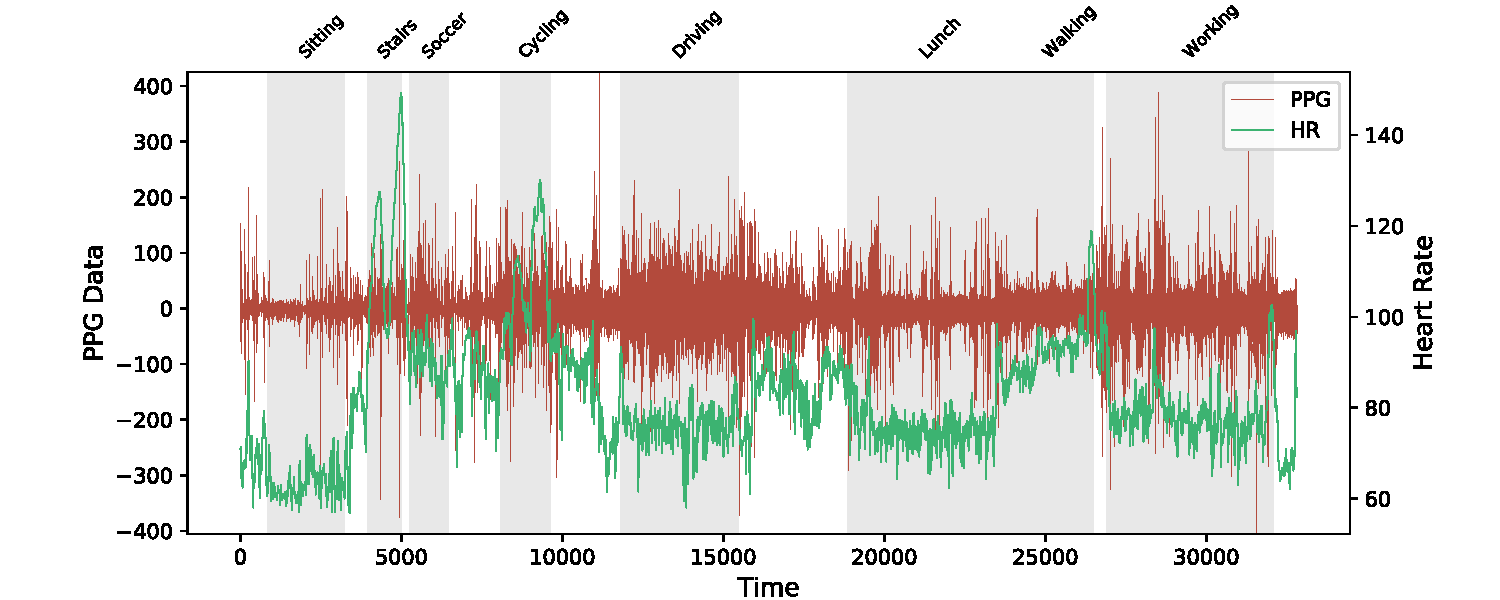
\includegraphics[width=7in]{image5}
  \caption{A visualization of the raw data from the PPG-DaLia: Subject 2’s BVP/PPG Data vs Heart Rate Ground Truth. Note the significant amount of noise in the BVP/PPG signal}
  \label{fig_1}
  \end{figure*}

\section{Methodology}

Reference \cite{reiss2019deep} provides the details about the data collection protocol. We have used the same steps as identified in the reference paper. This means we have segmented the time-series data with a sliding window of length 8 seconds and a window shift of 2 seconds. As core features, we made use of only the first PPG channel and accelerometer channels in the X, Y and Z axis. We may consider additional PPG channels as input for our deep learning model if model development and timing allow. As a second step, we applied Fast Fourier Transform (FFT) on each time-series segment. The result of this step is Nch = 4 channel time-frequency spectra, one per signal channel. In the next step, we cut these spectra, keeping only the 0–4 Hz interval (4 Hz corresponds to 240 bpm). The resulting number of FFT points per segment and channel is NFFT=1025. Finally, z-normalization (zero mean and unit variance) is performed on each channel’s spectrum. The final Nch time-frequency spectra serve as input for the deep learning model.

For the data preparation stage, we segmented the data with 8 seconds of sliding windows with a time rolling mechanism with 2 seconds shifts. This enabled us to extract features that we need from the data. Since we need both the time and frequency domain behavior of sensor channels, we extracted both time and frequency domain characteristics of each window. Time-domain characteristics include features indicating regularities and statistical measures on windows like mean, max, standard deviation, and unique/recurring value count, while frequency-domain features represent more complex, yet periodic information within each window. These features are FFT coefficients, number of CWT (continuous wavelet transform) peaks, and autoregression of each window. 

Since we were unsure about which features or characteristics will be most contrastive towards heart-rate estimation, we ended up extracting a large number of features from each window that we think might provide information to our model. However, this approach did lead to some correlation between features as well as some features that represent no information, which can be considered as noise. For this reason, we also applied univariate and multivariate feature selection techniques, which eliminated high correlation and noise features. 

After the selection procedures, we tried a variety of modeling procedures. We built a deep learning model similar to Reference \cite{reiss2019deep}, as well as simpler options like tree-based models, which allowed us to perform benchmarking on our additional features with easier training procedures. Moreover, such models let us understand the information value of the considered features without being much affected by scaling and correlation issues between input features. Here, our goal is to determine which features are beneficial for our task as well as which architecture is likely to give us the best results.
    
For the initial training, we have extracted both time and frequency domain features from the pre-processed 8 second time windows and benchmarked them on a subject basis. The features include simple extractions like mean, maximum, and standard deviation of acceleration values in each window, which are intended to capture the time domain characteristics of the features, while more complex features like FFT coefficients, autocorrelation, and linear trend capture frequency domain characteristics of the signals, which are especially important to predict heart rate in the presence of high-frequency acceleration dynamics, which are very common during movements and sports activities for each subject.

In parallel to the improved features, we implemented a model similar to the original CNN model from Reference \cite{reiss2019deep}. This allowed us to both implement the paper model itself, which is the minimum requirement for the project task, but also to build upon and improve the model itself with both architectural changes as well as new features, which we have experimented on in the initial training.

The performance metric is the same as the one used in \cite{reiss2019deep}, the mean absolute error (MAE) defined as:

\begin{equation}
	MAE=\frac{1}{W} \sum_{w=1}^{W} \lvert BPM_{est}(w)-BPM_{ref}(w) \rvert
\end{equation}

\section{Experiments}

Our initial target set at the start of the project was to achieve a lower or equal MAE than the reference paper \cite{reiss2019deep} on 6/9 Activities. We also compared the MAE results for our model with the session-wise evaluation results for the reference model.

Our initial results using the boosted-tree model on a subject-wise training yielded an MAE between 1.6 and 2.8, which is a significant improvement over the MAE recorded in the reference paper \cite{reiss2019deep}.  This improvement was the result of a simple gradient boosting model (XGBoost) without hyperparameter tuning. The evaluation was done by splitting each subject’s data on a standard 80:10:10 train-test-validate basis with 80\% of the data used for training. The initial results are presented in Table \ref{tab:table1}.

Here, the superior training results are achieved with the use of more complex time series features. Based on the extracted data windows, we have extracted 15 different features that represent the time and frequency domain characteristics of the heart-rate signals. Our features include simple series statistics like mean, variation coefficient (scaled variance), minimum and maximum as well as more complex frequency domain indicators like FFT and autoregressive characteristics. Here, the simple statistics capture the “mean heart rate” information from features while frequency domain indicators act like an implicit “activity recognition” model. These frequency domain features capture the activity, as well as the corresponding signal frequencies for each predicted activity for the current window. As such, our features performed superior to the paper features as our features are covering paper features and and more.
With these strong features, we have utilized a gradient boosting algorithm for benchmark purposes. The main reasons we chose XGBoost are as follows. First, it works well with large quantities of time series features, which inevitably have large correlation content. Since our feature pool is quite large, and generated features are from the same source, they carry some duplicate information content in the form of linear correlation. And since XGBoost is intrinsically a decision-tree based model, it does not get affected by high correlations and lets us perform the benchmarking. Secondly, since it is a boosting model, it performs well out of the box without requiring much tuning. For such models, the homogeneity of data is more important than the size, thus the model is allowing us to perform benchmarking of our features for the final model.

\begin{figure}[!t]
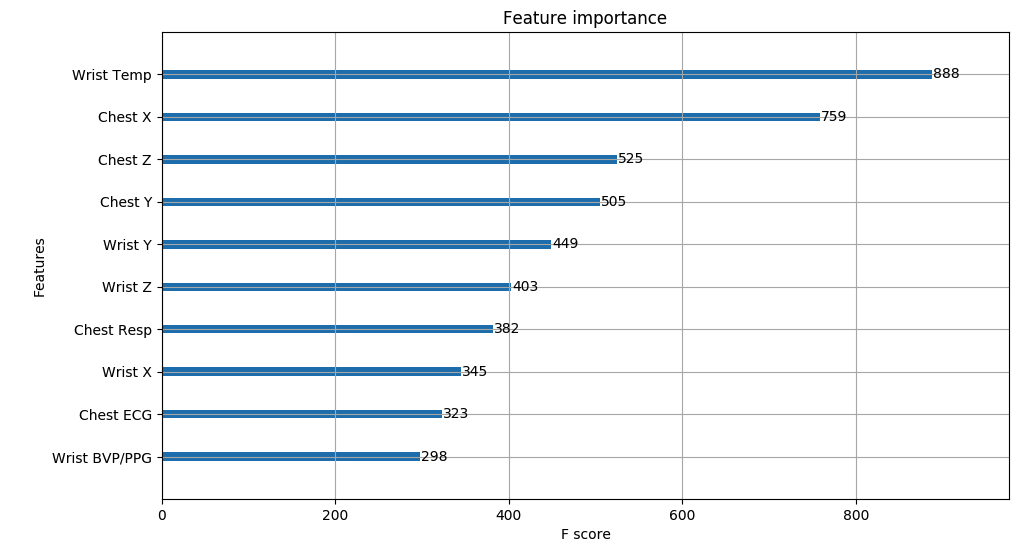
\includegraphics[width=3.5in]{image1}
\caption{A visualization of the untransformed feature importance ranking from the PPG-DaLia dataset relative to Ground Truth Heart Rate Prediction using Xgboost}
\label{fig_2}
\end{figure}

Subsequently, we built a convolutional neural network (CNN) similar to the model architecture proposed in Reference \cite{reiss2019deep}, in order to incorporate deep learning on activity-based training. The inputs to the deep learning model are four channels of time-frequency spectra corresponding to the x, y, and z accelerometer signals and the PPG signal (BVP), all collected from the wrist sensor.

The reference model \cite{reiss2019deep} has a deep CNN architecture with two initial convolution layers and up to 8 additional convolution-maxpool layers. The first two layers are designed to fuse first the input channels (accelerometer measurements and PPG), and the segments used in heart rate tracking, respectively. The successive convolution-maxpool layers are designed to increase the learning effectiveness of the model. One last convolutional layer is included in the model in order to reduce the input dimension of the fully connected layer. The last two layers are fully connected, with the first flattening the input and the second one providing a single value estimated heart rate. Note that the reference model also included a dropout layer which was also included in our model. Based on our evaluations the dropout layer can be omitted without significant effects on the model performance. The model uses an exponential linear unit (ELU) as activation function for all the layers. The loss function is defined as the Mean Squared Error (MSE) between the estimated value for a given segment and the corresponding ground truth. For optimization the model uses the Adam optimizer \cite{kingma2014adam}. We included the same filter size as the reference model to decrease the spatial size of the output. This decreased the number of features volume but increased the depth of the volume. The reference paper mentioned that this technique has been successfully implemented in other architectures like VGGNet, ResNet, and DenseNet \cite{reiss2019deep}. 
Similar to the reference paper, we implemented multiple scenarios to try and improve the network architecture. We tried ReLU activation function, different optimizers, and loss functions to try to improve model performance. In addition, we implemented different CNN layers with smaller filters to try and pick up finer detail. However, it seems though the initial CNN architecture similar to the paper \cite{reiss2019deep} is already well set and any of the changes did not improve or otherwise drastically worsen the MAE score. We determined in the end to implement a deep learning model architecture similar to the reference paper to determine if the preprocessing and additional activity prediction would help our overall MAE score.  
Our initial model replicated the reference network architecture in \cite{reiss2019deep} as described above. An illustration of the architecture is provided in Figure \ref{fig_3} - note that the figure also shows the predicted activity used as input in the final model (see below) but not in the initial model. The model was trained using a 80:20 train-test data split. The results from the initial model were rather disappointing as the performance of our model in terms of MAE was significantly higher than the reference model. Our initial model had higher MAE for almost all subjects and an average MAE of 13.37 $\pm$ 3.1 BPM, compared to the reference model average MAE of 7.65 $\pm$ 4.2 BPM.

To improve the model performance we initially envisioned the use of additional features we benchmarked in the initial training, which have performed very well. This included the development of an ensemble architecture that includes a simple activity recognition model. The activity is very important in the HR estimation and it is usually not explicitly available as an input to the model, thus it was identified early as a candidate to incorporate for model improvement, which we noted was proposed in some other works as well \cite{brophy2020optimised}. Moreover, we are aware that the interpretability aspect of the model is crucial for both improving and approval of it. We have performed a literature search on the interpretability aspect and found the SHAP algorithm \cite{lundberg2017unified}, which can help us with the interpretation aspect of the model.

\begin{figure*}[!t]
  \centering
  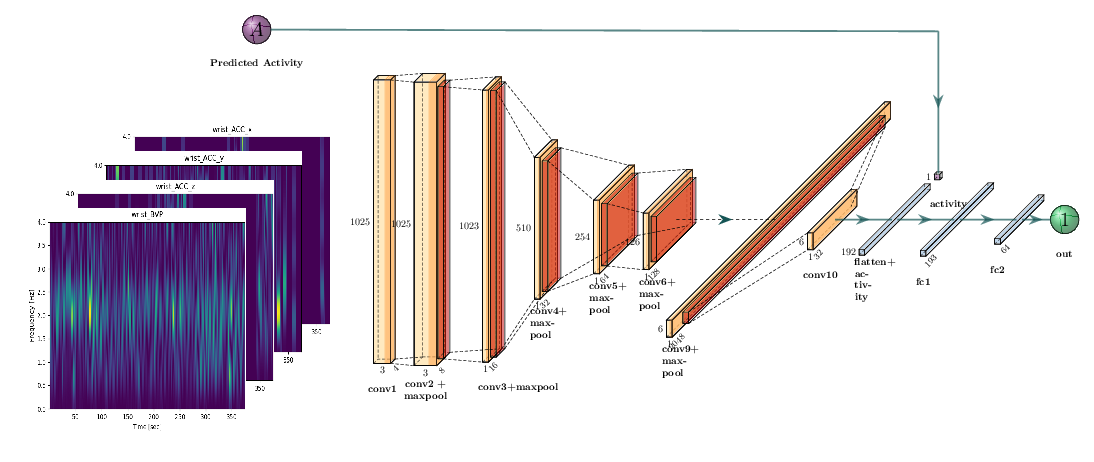
\includegraphics[width=7in]{image4}
  \caption{Network architecture for the proposed model. The initial model did not include the predicted activity shown at the top. The predicted activity was included in the final model and is generated externally using an additional predictive model.}
  \label{fig_3}
  \end{figure*}

Several model changes were implemented in order to improve the model performance. The most significant improvement was the addition of the predicted activity as a feature using an additional prediction model. Here, we have developed an ensemble approach to prediction by training a “hypermodel” that is specifically trained for recognizing the user’s current activity. The model is a lightweight Random Forest model developed for the multi-class classification task of activity recognition. It is feasible to be used in real-time in user’s worn devices, and only uses the sensor data that is available in the wrist device, which are acceleration and BVP. Using this data in real-time, we have achieved between 87\%-95\% accuracy for activity prediction among subjects. Essentially, it has become a surrogate model for the main HR predictor, allowing the model to contrast better between activities and make more accurate predictions. The surrogate model decreased our mean MAE results, but more importantly, it has greatly decreased the standard deviation of errors, allowing the model to make much more stable predictions over the relatively more homogeneous partitioned data, as expected.

\begin{figure*}[!t]
\centering
\subfloat[Subject 2]{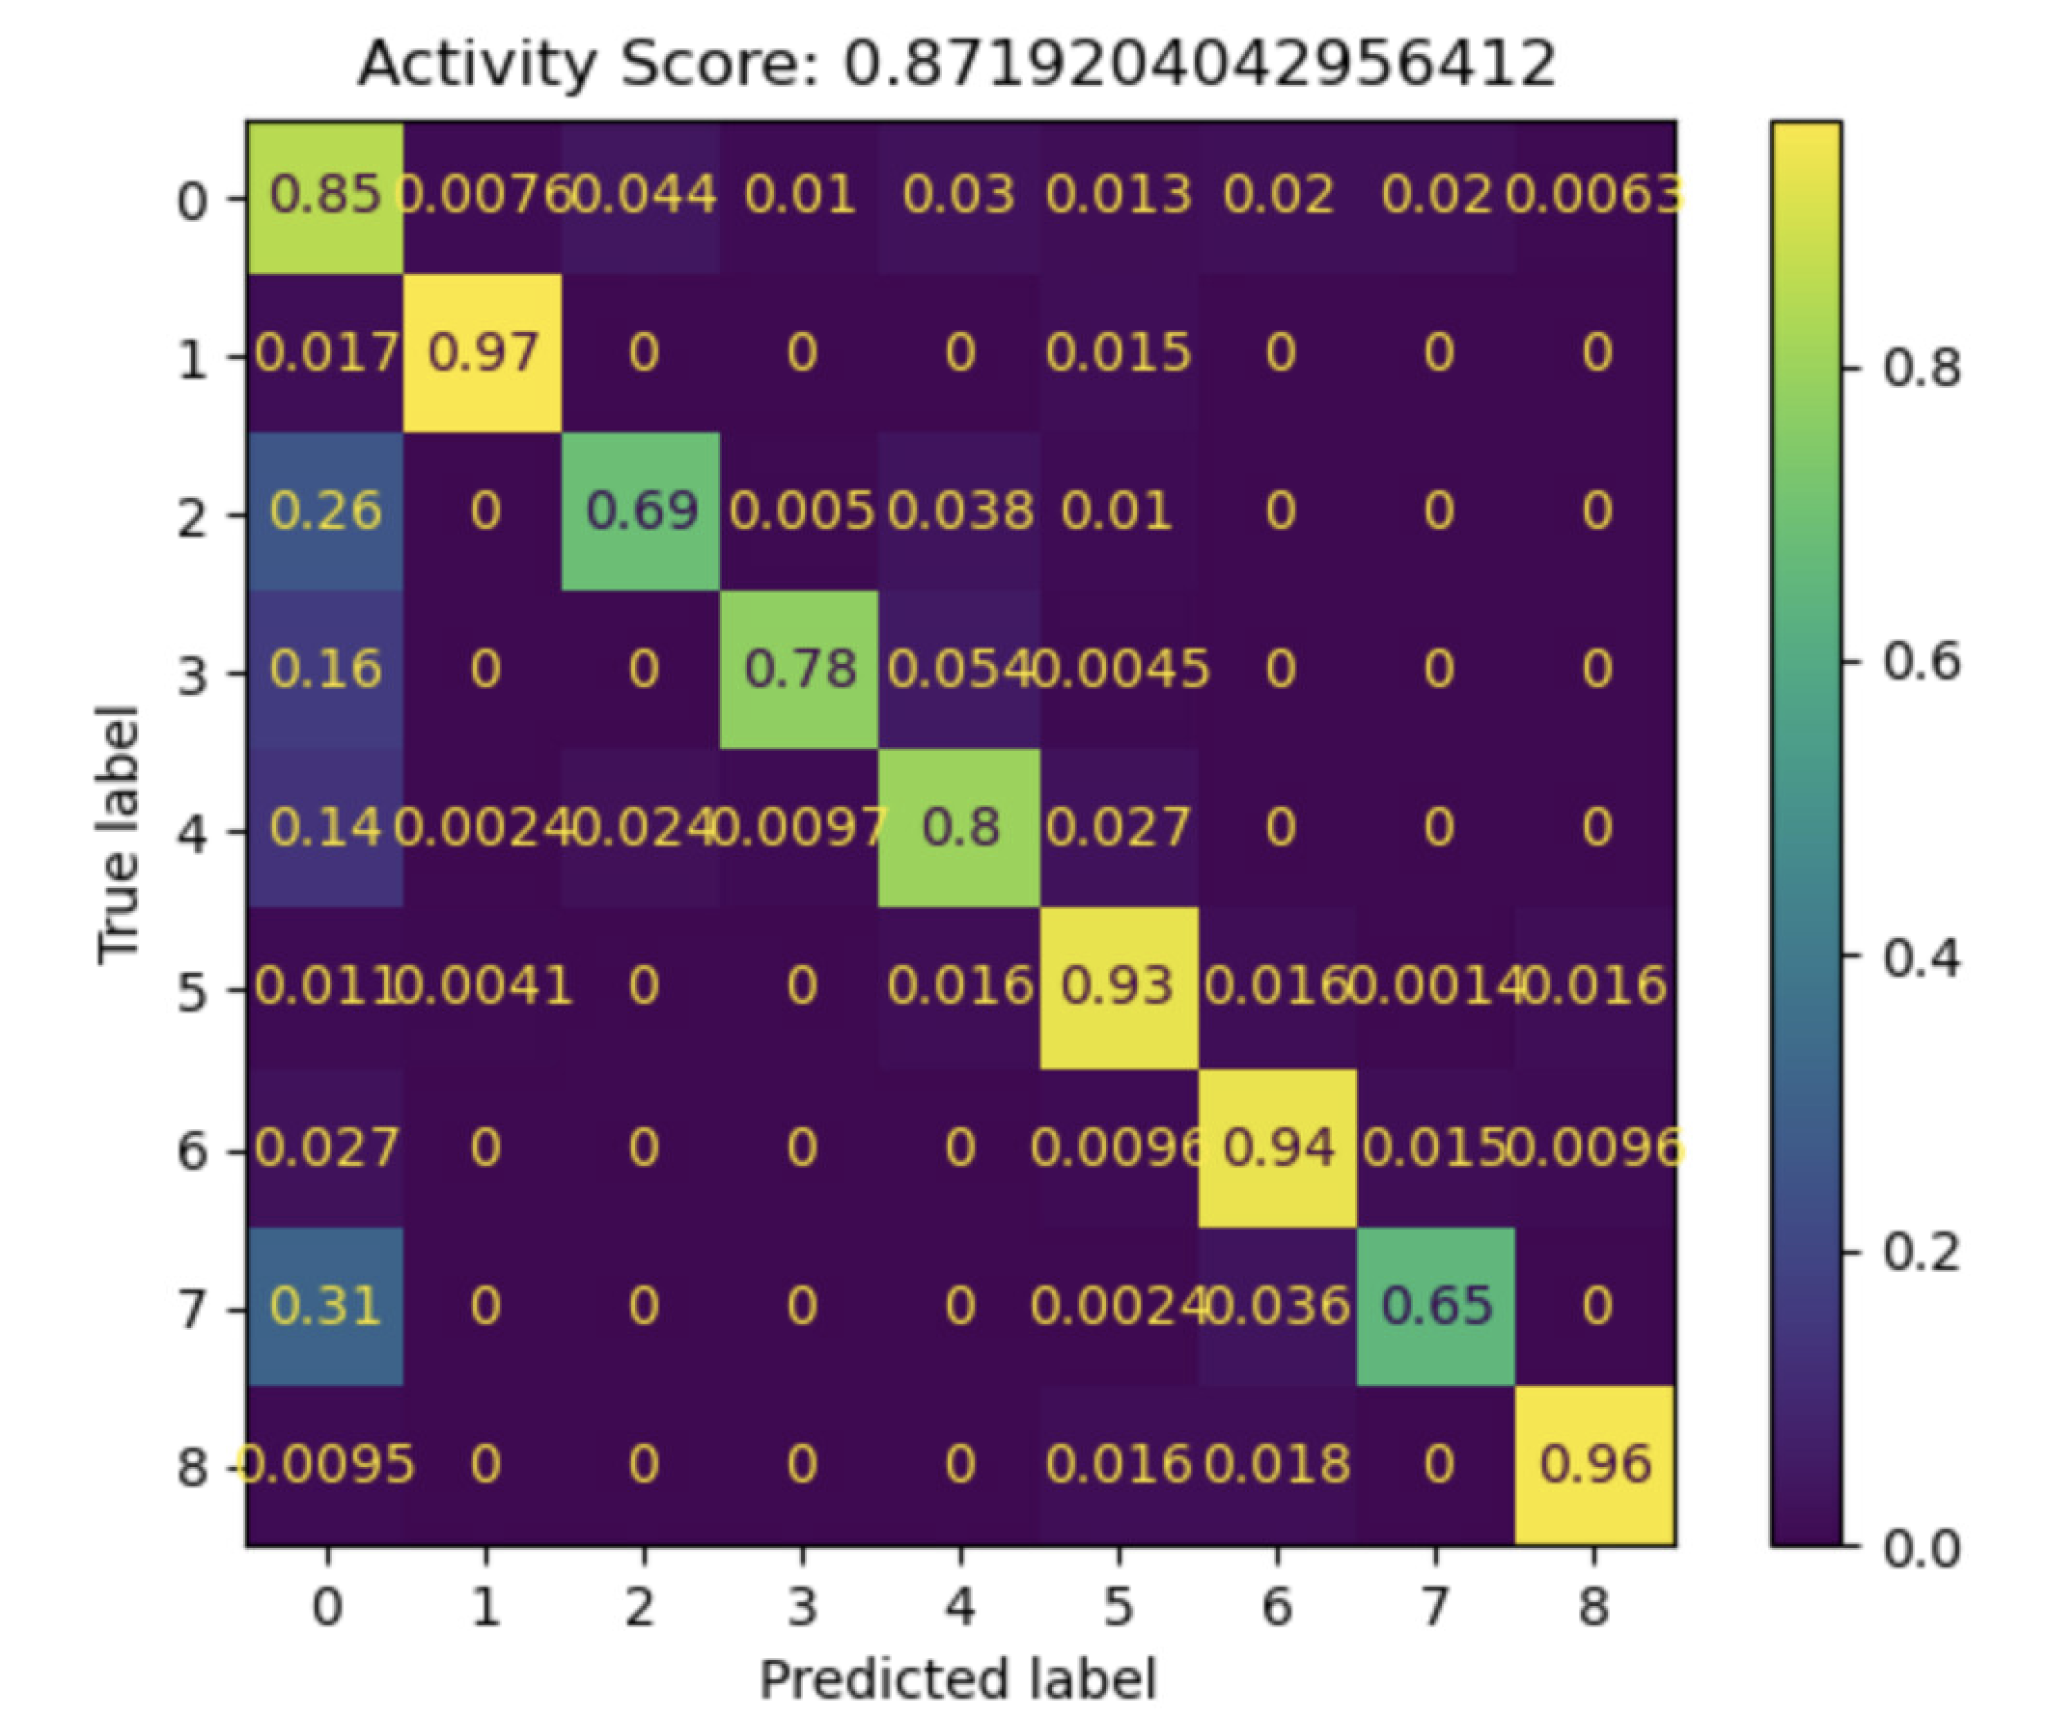
\includegraphics[width=2.5in]{image3}%
\label{fig_4a}}
\hfil
\subfloat[Subject 12]{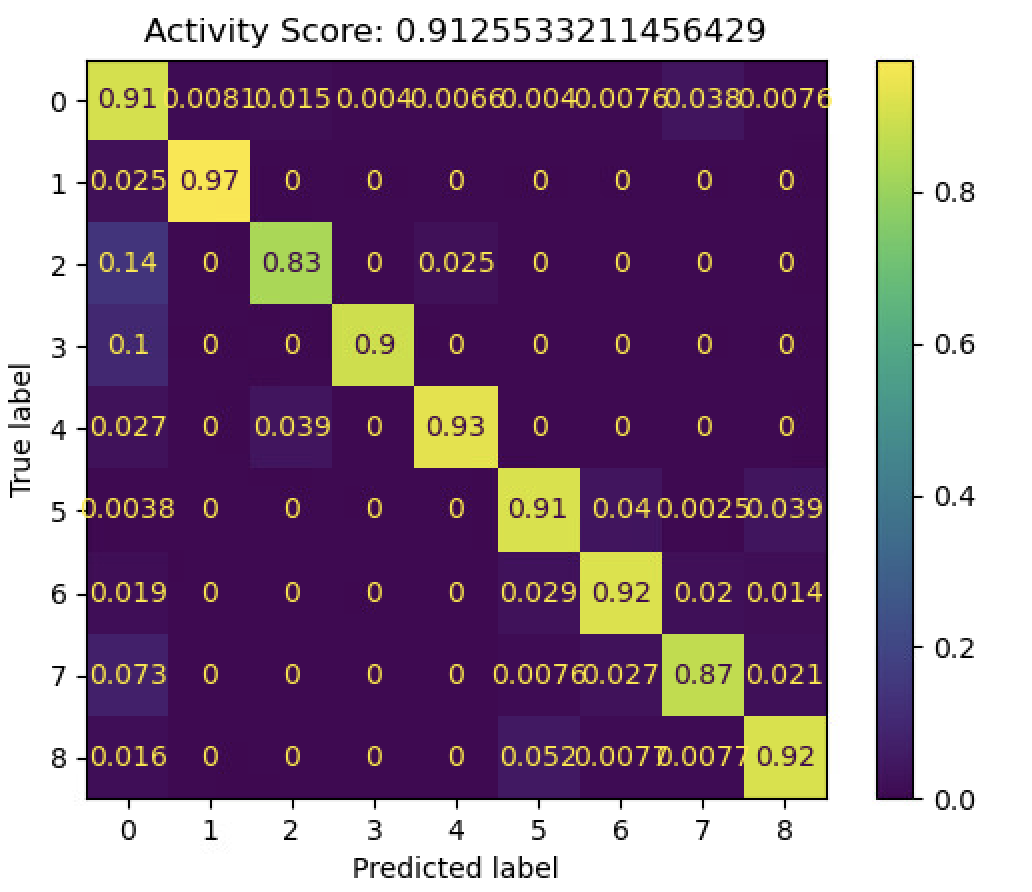
\includegraphics[width=2.5in]{image2}%
\label{fig_4b}}
\caption{Activity prediction model performance for Subject 2 (a) and Subject 12 (b). Most of the confusion is  between transition actions (Label 0) and stairs climbing (Label 2) and table tennis (Label 3) as expected.}
\label{fig_4}
\end{figure*}

In this final configuration, the model performance was greatly improved compared to the initial model. Improvements were also evident in comparison to the reference model in \cite{reiss2019deep}, in particular for the activities where the heart rates are elevated compared to the baseline (e.g. sport activities). Table \ref{tab:table1} shows the comparison of the results obtained. Our ensemble model with activity prediction had similar or better MAE for most subjects and an average MAE of 7.33 $\pm$ 1.15 BPM, compared to the reference model average MAE of 7.65 $\pm$ 4.2 BPM. Improvements were noted in particular for the activities where the heart rates are elevated compared to the baseline (e.g. sport activities). We also note that our ensemble model performance is more consistent between subjects and has significantly lower variability compared to the reference model.


\begin{table*}[t] 
  \tiny
  \centering
  \caption{Comparison of results for our models with the reference}\label{tab:table1}
  \tabulinesep = 1mm
  \begin{tabu} to\linewidth {X[2,l,m]X[1,c,m]X[1,c,m]X[1,c,m]X[1,c,m]X[1,c,m]X[1,c,m]X[1,c,m]X[1,c,m]X[1,c,m]X[1,c,m]X[1,c,m]X[1,c,m]X[1,c,m]X[1,c,m]X[1,c,m]X[2,c,m]}
  \toprule
  \textbf{Subject} & \textbf{S1}& \textbf{S2} & \textbf{S3} & \textbf{S4} & \textbf{S5}& \textbf{S6}& \textbf{S7}& \textbf{S8}& \textbf{S9}& \textbf{S10}& \textbf{S11}& \textbf{S12}& \textbf{S13}& \textbf{S14}& \textbf{S15}& \textbf{All}\\
  \midrule
  \textbf{Reference CNN Average}& 8.45 & 7.92 & 5.96 & 7.86 & 18.97 & 13.55 & 5.16 & 11.49 & 10.65 & 6.07 & 9.87 & 9.95 & 5.25 & 5.85 & 5.25 & 8.82 $\pm$ 3.8 \\
  \textbf{Reference CNN Ensemble}& 7.73 & 6.74 & 4.03 & 5.9 & 18.51 & 12.88 & 3.91 & 10.87 & 8.79 & 4.03 & 9.22 & 9.35 & 4.29 & 4.37 & 4.17 & 7.65 $\pm$ 4.2 \\
  \textbf{Gradient Boosting (Xgboost)}& 2.32 & 2.1 & 2.3 & 2.22 & 2.13 & 2.43 & 2.58 & 2.29 & 2.11 & 1.94 & 2.85 & 1.64 & 2.7 & 2.83 & 2.03 & 2.30 $\pm$ 0.34 \\
  \textbf{Initial CNN Model}& 12.13 & 9.91 & 11.99 & 9.55 & 15.38 & 17.80 & 13.28 & 8.62 & 15.30 & 11.38 & 18.65 & 11.14 & 17.56 & 13.76 & 14.16 & 13.37 $\pm$ 3.10 \\
  \textbf{Ensemble CNN with Activity Prediction} & 7.24  & 7.09 & 7.81 & 6.30 & 7.25 & 7.71 & 7.36 & 5.46 & 7.49 & 7.51 & 9.38 & 5.61 & 9.48 & 8.03 & 6.24 & 7.33 $\pm$ 1.15 \\
  \bottomrule
  \end{tabu}
  \end{table*}%

Data processing was performed on our own individual computers with a processing time of around 15 minutes for all the subjects for general processing and around 45 minutes for all the subjects for FFT transform and normalization on a Core i7 Intel processor with 32 GB of RAM running Linux kernel 4.15.0. Training of the deep learning models was mostly performed on \url{lambdalabs.com} GPU cloud instances varying from 2xA6000 48 GB RAM 28 vCPU to 8x Tesla V100 16 GB RAM 92 vCPU. Training time ranged from ~25 minutes to ~65 minutes depending on the model and the training instance selected.

We cannot conclude without noting the significant better performance of the boosted tree model (XGBoost) compared to all the other models evaluated. Not only did the boosted tree model outperform all the other models in all the categories, but it did so with much lower MAE (average of  2.30 $\pm$ 0.34 BPM) and without any tuning. It is generally difficult to explain and justify how predictions are made with a neural network model. In contrast, a decision tree is easily explained, and the  decision “workflow” through the decision tree can be readily implemented as a logical algorithm. For these reasons, we find that a tree model may be better suited and easier to implement as a predictive model for PPG-based heart rate predictions in wearable devices.

\section{Conclusion}

In this paper, we sought to improve a state-of-the-art heart rate deep-learning prediction algorithm. One of the primary innovations to this end was the preprocessing of various non-linear statistical features of the time-segmented windows of signals in order to get an equal or lower MAE score during evaluation of our model and the implementation of an ensemble model with an activity prediction. The preprocessed features took significant time to implement due to the size of the raw data and the filtering of the discrepancies that occur. The preprocessed data included FFT coefficients, autocorrelation, and linear trend capture frequency domain characteristics. Using the preprocessed features in a given window size, we were able to prove that the features were beneficial using a preliminary testing with XGBoost. We replicated the CNN model in Reference \cite{reiss2019deep}, and tried other deep learning architectures to lower the MAE score. Our ensemble CNN model matched or exceeded the performance of the reference CNN model from Reference \cite{reiss2019deep}. Our boosted-tree model performed significantly better than any model we compared to, and we recommend it for use because it is generally easier to explain and to implement in wearable devices.

\section*{Resources}

\paragraph*{Github repository for our code} \small{\url{https://github.com/denizhankara/PPG-DaLiA}}\\

\paragraph*{Project contributions (in alphabetical order)}

\begin{itemize}
\item Andrei Burghelea - Input Data Preparation, Model Architecture, Model Training, Documentation
\item David Gutierrez - Data Visualization, Documentation, Research Structure
\item Denizhan Kara - Input Data Preparation, Model Training, Documentation
\item Sung Yoo Kim - Model Architecture, Model Training, Documentation
\end{itemize}




% An example of a floating figure using the graphicx package.
% Note that \label must occur AFTER (or within) \caption.
% For figures, \caption should occur after the \includegraphics.
% Note that IEEEtran v1.7 and later has special internal code that
% is designed to preserve the operation of \label within \caption
% even when the captionsoff option is in effect. However, because
% of issues like this, it may be the safest practice to put all your
% \label just after \caption rather than within \caption{}.
%
% Reminder: the "draftcls" or "draftclsnofoot", not "draft", class
% option should be used if it is desired that the figures are to be
% displayed while in draft mode.





% Note that the IEEE typically puts floats only at the top, even when this
% results in a large percentage of a column being occupied by floats.


% An example of a double column floating figure using two subfigures.
% (The subfig.sty package must be loaded for this to work.)
% The subfigure \label commands are set within each subfloat command,
% and the \label for the overall figure must come after \caption.
% \hfil is used as a separator to get equal spacing.
% Watch out that the combined width of all the subfigures on a 
% line do not exceed the text width or a line break will occur.
%
%\begin{figure*}[!t]
%\centering
%\subfloat[Case I]{\includegraphics[width=2.5in]{box}%
%\label{fig_first_case}}
%\hfil
%\subfloat[Case II]{\includegraphics[width=2.5in]{box}%
%\label{fig_second_case}}
%\caption{Simulation results for the network.}
%\label{fig_sim}
%\end{figure*}
%
% Note that often IEEE papers with subfigures do not employ subfigure
% captions (using the optional argument to \subfloat[]), but instead will
% reference/describe all of them (a), (b), etc., within the main caption.
% Be aware that for subfig.sty to generate the (a), (b), etc., subfigure
% labels, the optional argument to \subfloat must be present. If a
% subcaption is not desired, just leave its contents blank,
% e.g., \subfloat[].


% An example of a floating table. Note that, for IEEE style tables, the
% \caption command should come BEFORE the table and, given that table
% captions serve much like titles, are usually capitalized except for words
% such as a, an, and, as, at, but, by, for, in, nor, of, on, or, the, to
% and up, which are usually not capitalized unless they are the first or
% last word of the caption. Table text will default to \footnotesize as
% the IEEE normally uses this smaller font for tables.
% The \label must come after \caption as always.
%
%\begin{table}[!t]
%% increase table row spacing, adjust to taste
%\renewcommand{\arraystretch}{1.3}
% if using array.sty, it might be a good idea to tweak the value of
% \extrarowheight as needed to properly center the text within the cells
%\caption{An Example of a Table}
%\label{table_example}
%\centering
%% Some packages, such as MDW tools, offer better commands for making tables
%% than the plain LaTeX2e tabular which is used here.
%\begin{tabular}{|c||c|}
%\hline
%One & Two\\
%\hline
%Three & Four\\
%\hline
%\end{tabular}
%\end{table}


% Note that the IEEE does not put floats in the very first column
% - or typically anywhere on the first page for that matter. Also,
% in-text middle ("here") positioning is typically not used, but it
% is allowed and encouraged for Computer Society conferences (but
% not Computer Society journals). Most IEEE journals/conferences use
% top floats exclusively. 
% Note that, LaTeX2e, unlike IEEE journals/conferences, places
% footnotes above bottom floats. This can be corrected via the
% \fnbelowfloat command of the stfloats package.




%\section{Conclusion}
%The conclusion goes here.





% if have a single appendix:
%\appendix[Proof of the Zonklar Equations]
% or
%\appendix  % for no appendix heading
% do not use \section anymore after \appendix, only \section*
% is possibly needed

% use appendices with more than one appendix
% then use \section to start each appendix
% you must declare a \section before using any
% \subsection or using \label (\appendices by itself
% starts a section numbered zero.)
%


%\appendices
%\section{Proof of the First Zonklar Equation}
%Appendix one text goes here.

% you can choose not to have a title for an appendix
% if you want by leaving the argument blank
%\section{}
%Appendix two text goes here.


% use section* for acknowledgment
%\section*{Acknowledgment}


%The authors would like to thank...


% Can use something like this to put references on a page
% by themselves when using endfloat and the captionsoff option.
\ifCLASSOPTIONcaptionsoff
  \newpage
\fi



% trigger a \newpage just before the given reference
% number - used to balance the columns on the last page
% adjust value as needed - may need to be readjusted if
% the document is modified later
%\IEEEtriggeratref{8}
% The "triggered" command can be changed if desired:
%\IEEEtriggercmd{\enlargethispage{-5in}}

% references section

% can use a bibliography generated by BibTeX as a .bbl file
% BibTeX documentation can be easily obtained at:
% http://mirror.ctan.org/biblio/bibtex/contrib/doc/
% The IEEEtran BibTeX style support page is at:
% http://www.michaelshell.org/tex/ieeetran/bibtex/
%\bibliographystyle{IEEEtran}
% argument is your BibTeX string definitions and bibliography database(s)
%\bibliography{IEEEabrv,../bib/paper}
%
% <OR> manually copy in the resultant .bbl file
% set second argument of \begin to the number of references
% (used to reserve space for the reference number labels box)
%\begin{thebibliography}{1}
%
%\bibitem{DeepPPG:reiss}
%	A.~Reiss, I.~Indlekofer, P.~Schmidt and K.~Van~Laerhoven. \emph{Deep PPG: Large-scale heart rate estimation with convolutional neural networks}. \hskip 1em plus
%  0.5em minus 0.4em\relax Sensors, 19(14):3079.
%\end{thebibliography}

\bibliographystyle{ieeetran}
\bibliography{references}


% biography section
% 
% If you have an EPS/PDF photo (graphicx package needed) extra braces are
% needed around the contents of the optional argument to biography to prevent
% the LaTeX parser from getting confused when it sees the complicated
% \includegraphics command within an optional argument. (You could create
% your own custom macro containing the \includegraphics command to make things
% simpler here.)
%\begin{IEEEbiography}[{\includegraphics[width=1in,height=1.25in,clip,keepaspectratio]{mshell}}]{Michael Shell}
% or if you just want to reserve a space for a photo:

%\begin{IEEEbiography}{Michael Shell}
%Biography text here.
%\end{IEEEbiography}

% if you will not have a photo at all:
%\begin{IEEEbiographynophoto}{John Doe}
%Biography text here.
%\end{IEEEbiographynophoto}

% insert where needed to balance the two columns on the last page with
% biographies
%\newpage

%\begin{IEEEbiographynophoto}{Jane Doe}
%Biography text here.
%\end{IEEEbiographynophoto}

% You can push biographies down or up by placing
% a \vfill before or after them. The appropriate
% use of \vfill depends on what kind of text is
% on the last page and whether or not the columns
% are being equalized.

%\vfill

% Can be used to pull up biographies so that the bottom of the last one
% is flush with the other column.
%\enlargethispage{-5in}



% that's all folks
\end{document}


